\documentclass[a4paper,10pt]{article}
\usepackage[french]{babel}
\usepackage[utf8]{inputenc}
\usepackage[left=2.5cm,top=2cm,right=2.5cm,nohead,nofoot]{geometry}
\usepackage{url}
\usepackage{graphicx}
\usepackage{float}
\usepackage[colorinlistoftodos]{todonotes}
\usepackage{hyperref}
\usepackage{amssymb}
\usepackage{dsfont}
\usepackage{amsmath}

\linespread{1.1}



\begin{document}

\begin{titlepage}
\begin{center}
\textbf{\textsc{UNIVERSIT\'E DE MONTR\'EAL}}\\
%\textbf{\textsc{Faculté des Sciences}}\\
%\textbf{\textsc{Département d'Informatique}}
\vfill{}\vfill{}
\begin{center}{\Huge Rapport : Devoir1 }\end{center}{\Huge \par}
\begin{center}{\large Pierre Gérard \\ Mathieu Bouchard}\end{center}{\Huge \par}
\vfill{}\vfill{} \vfill{}
\begin{center}{\large \textbf{IFT3395-6390 Fondements de l'apprentissage machine}}\hfill{\\Pascal Vincent, Alexandre de Brébisson et César Laurent}\end{center}{\large\par}
\vfill{}\vfill{}\enlargethispage{3cm}
\textbf{Année académique 2015~-~2016}
\end{center}
\end{titlepage}

%\begin{abstract}
%Ce rapport présente ...
%\end{abstract}


\tableofcontents

\pagebreak

\section{Partie Théorique : Estimation de densité}

\subsection{Densité avec des fenêtres de Parzen a noyau Gaussien isotropique}

a) $\mathcal{N}_{x^{(i)}, \sigma^{2}} = \frac{1}{(2 \pi)^{d/2} \sigma^{d}} e^{ \frac{-1}{2} \frac{d(x^{i},x)^{2}}{\sigma^{2}} } $



b) Si on choisit de prendre tous les points du voisinages
$ p(x) =  \frac{1}{n} \sum_{i=1}^{n} \mathcal{N}_{x^{(i)}, \sigma^{2}} $
\todo{distribuer pour virer la somme?}

c) Hyper-paramètre: $\sigma \in \mathds{R}$

Paramètre : On mémorise l'ensemble des données d'entrainement. $( n \times \mathds{R}^{d})$

On considère cette méthode comme non-paramétrique car le nombre de paramètre varie avec la taille de l'ensemble de données.



d)
\todo{Le petit d}
3 propriété a prouvé: integral, integral=1, toujours positive (ou presque)

\subsection{Densité paramétrique avec Gaussienne isotropique}

a) $p(x) = \frac{1}{(2 \pi)^{d/2} \sigma^{d}} e^{\frac{-\mid\mid x- \mu \mid\mid ^{2}}{2 \sigma^{2}} }$


$\mu$ est le est le vecteur des moyennes, de dimension d.
$\Sigma$ est la matrice de covariance, de dimension 1.



b) Dans le cas de l'estimation par fenêtre de Parzen, il nous faut effectuer une moyenne sur n densités Gaussiennes et, pour chacune d'elles, le point x(i) sert de moyenne $\mathcal{N}_{x^{(i)}, \sigma^{2}}$ avec $\sigma$ qui est un hyperparamètre. Dans le cas présent, on utilise une seule densité Gaussienne pour laquelle il faudra apprendre les valeurs de moyenne $\mu$ et d'écart-type $\sigma$.

c)

Paramètres :
\begin{itemize}
	\item $\mu$ est le est le vecteur des moyennes, de dimension d.
	\item $\Sigma$ est la matrice de covariance, de dimension 1.
\end{itemize}

Pas d'hyper-paramètre.


\subsection{Densité paramétrique avec Gaussienne diagonale}

a) $p(x) = \frac{1}{(2 \pi)^{d/2} \sqrt{\mid{\Sigma} \mid}} e^{\frac{-1}{2} (x- \mu)^{T} \Sigma^{-1} (x- \mu) }$
\begin{itemize}
	\item $\mu$ est le est le vecteur des moyennes, de dimension d.
	\item $\Sigma$ est la matrice de covariance, de dimension d.
\end{itemize}

\[
\Sigma =
\begin{bmatrix}
    \sigma_{1} & 0 & 0 & \dots  & 0 \\
    0 & \sigma_{2} & 0 & \dots  & 0 \\
    \vdots & \vdots & \vdots & \ddots & \vdots \\
    0 & 0 & 0 & \dots  & \sigma_{n}
\end{bmatrix}
\]

b)Indépendance des composantes d'un vecteur aléatoire suivant une distribution Gaussienne diagonale :

Soit $x \in \mathds{R}^{d}$ un vecteur aléatoire qui suit une distribution Gaussienne diagonale $\mathcal{N}_{\mu , \sigma(x)}$

Posons $x - \mu = k$ et $\frac{1}{(2 \pi)^{d/2} \sqrt{\mid{\Sigma} \mid}} = s$
\[
\Sigma =
\begin{bmatrix}
    \sigma_{1} & 0 & 0 & \dots  & 0 \\
    0 & \sigma_{2} & 0 & \dots  & 0 \\
    \vdots & \vdots & \vdots & \ddots & \vdots \\
    0 & 0 & 0 & \dots  & \sigma_{n}
\end{bmatrix}
\Sigma^{-1} =
\begin{bmatrix}
    \frac{1}{\sigma_{1}} & 0 & 0 & \dots  & 0 \\
    0 & \frac{1}{\sigma_{2}} & 0 & \dots  & 0 \\
    \vdots & \vdots & \vdots & \ddots & \vdots \\
    0 & 0 & 0 & \dots  & \frac{1}{\sigma_{n}}
\end{bmatrix}
\]

$p(x) = \mathcal{N}_{\mu , \Sigma(x)} = \frac{1}{(2 \pi)^{d/2} \sqrt{\mid{\Sigma} \mid}} e^{\frac{-1}{2} (x- \mu)^{T} \Sigma^{-1} (x- \mu) } = s \times e^{\frac{-1}{2} k^{t} \Sigma^{-1} k }$

$p(x) = s \times e^{\frac{-1}{2} (\frac{k_{1}}{\sigma_{1}^{2}} \frac{k_{2}}{\sigma_{2}^{2}} ... \frac{k_{d}}{\sigma_{d}^{2}} )k }  = s \times e^{\frac{-1}{2} \sum_{i=1}^{d} \frac{k_{i}^{2} }{\sigma_{i}^{2}} }$

$p(x) = s \prod_{i=1}^{d} e^{\frac{-1}{2} \frac{k_{i}^{2} }{\sigma_{i}^{2}} }  = s \prod_{i=1}^{d} e^{\frac{-1}{2} (x^{i} - \mu)^{T} \Sigma^{-1} (x^{i} - \mu) } $ où $x^{i}$ est un vecteur de taille $d$ avec la $i^{eme}$ valeur de $x$ en position $i$ et des 0 partout ailleurs.

$p(x) =\frac{1}{(2 \pi)^{d/2} \sqrt{\mid{\Sigma} \mid}} \prod_{i=1}^{d} e^{\frac{-1}{2} (x^{i} - \mu)^{T} \Sigma^{-1} (x^{i} - \mu) }  $

$p(x) = \prod_{i=1}^{d} p(x^{i}) $


La densité estimée pour à partir d'un vecteur aléatoire $x \in R$ qui suit une distribution gaussienne diagonale est égale au produit des densités estimées des composantes de ce vecteur aléatoire. On peut en conclure que ces composantes sont des variables aléatoires indépendantes.


c) \todo{gd c}

d) \todo{gd d}


\subsection{Choix du modèle}

La première tâche à effectuer pour choisir le modèle le plus approprié est de sélectionner un ensemble de tous les modèles que nous pourrions effectuer. Ici, il s'agit des approches présentées aux sections 1.1, 1.2 et 1.3. Ensuite, pour chacun des modèles sélectionnées, on procède ainsi :

\begin{enumerate}
	\item Soit $A$ , le modèle courant.
	\item Si le modèle contient des hyper-paramètres, répéter la procédure pour toutes les valeurs acceptables que ces hyper-paramètres peuvent prendre. Appelons cette configuration $\lambda$. Rappelons que l'approche des fenêtres de Parzen à noyau isotropique contient un hyper- paramètre (l'écart-type $\sigma$) tandis que les approches 2 et 3 n'en n'ont aucun ( $\lambda= \O$ ).
	\item Mélanger les éléments de l'ensemble $D$ s'ils étaient ordonnés.
	\item Séparer l'ensemble d'entraînement $D$ en deux sous-ensembles $D_{train}$ et $D_{valid}$. L'ensemble d’entraînement devrait être plus grand que l'ensemble de validation. $x \in \mathds{R}$ qui suit une distribution Gaussienne
	\item Entraîner $A$ avec la configuration d'hyper-paramètres choisis sur l'ensemble d'entraînement. On obtient alors : $\widehat{f} (A_{\lambda})=A_{\lambda}(D_{train})$
	\item Evaluer le résultat à l'aide de l'ensemble de validation. $e_{(A_{\lambda})} = \widehat{R} ( \widehat{f}_{(A_{\lambda})} , D_{valid} )$
\end{enumerate}

Une fois que ce travail a été effectuer pour tous les algorithmes et, pour chacun, sur chaque configurations d'hyper-paramètres $\lambda$ jugés admissibles, on regarde les valeurs de $e_{(A_{\lambda})}$ obtenues. Le modèle $A_{\lambda}$ qui retourne une erreur de validation minimale $e*_{A_{\lambda}}$ sera alors sélectionner. 
Nous aurions également pu séparer $D$ en 3 sous-ensembles plutôt que 2 et ainsi ajouter un ensemble de test. Une fois l'algorithme optimal trouvé à l'aide de l'ensemble d'entraînement et de l'ensemble de validation, nous aurions pu calculer un estimé non-biaisé de la performance de généralisation de l'algorithme choisit en calculant l'erreur empirique de validation sur l'ensemble de test; soit un ensemble de données dont le valeurs n'ont jamais été utilisées pour sélectionner l'algorithme dans les étapes précédantes. Cette étape nous permet de nous assurer (si nous avons assez de donner pour pouvoir effectuer un test concluent) que l'algorithme sélectionné est capable de généraliser sur de nouvelles données et qu'il n'est pas juste efficace sur les données de $D_{train}$ et $D_{valid}$.



\section{Partie Théorique : Classifieurs de Bayes}

\subsection{Classifieur de Bayes obtenu avec des densités paramétriques Gaussiennes diagonales}

a)Pour la probabilité a postériori.
\begin{itemize}
	\item $\mu$ est le est le vecteur des moyennes, de dimension d.
	\item $\Sigma$ est la matrice de covariance, de dimension d.
\end{itemize}
Pour la probabilité a priori.
\begin{itemize}
	\item $\mu$ la proportion d'element de chaque classe, de dimension m.
\end{itemize}

b)

c)
$P(Y=c | X=x)  = \frac{P(X=x | Y=c) P(Y=c)}{P(X=x)} $

$P(Y=c | X=x)  = \frac{ p_{c}(x) P_{c}}{p_{c'} P_{c'} } $

\subsection{Classifieur de Bayes obtenu avec des fenêtres de Parzen à noyau Gaussien isotropique}

a)

b)


\subsection{Classifieur de Bayes obtenu avec des fenêtres de Parzen à noyau Gaussien isotropique}

a)

b)

\section{Implémentation}

Pour tester notre code et l'implémentation, exécuter simplement dans le dossier $src$ :
\begin{verbatim}
	python main.py
\end{verbatim}
L'ensemble des graphiques vont être sauvé comme image.

Note : Les modules suivants utilisé en labo sont nécessaire : numpy, matplotlib, pylab.


\section{Partie Pratique : Estimation de densité}

\subsection{Densité 1D}

\begin{figure}[H]
	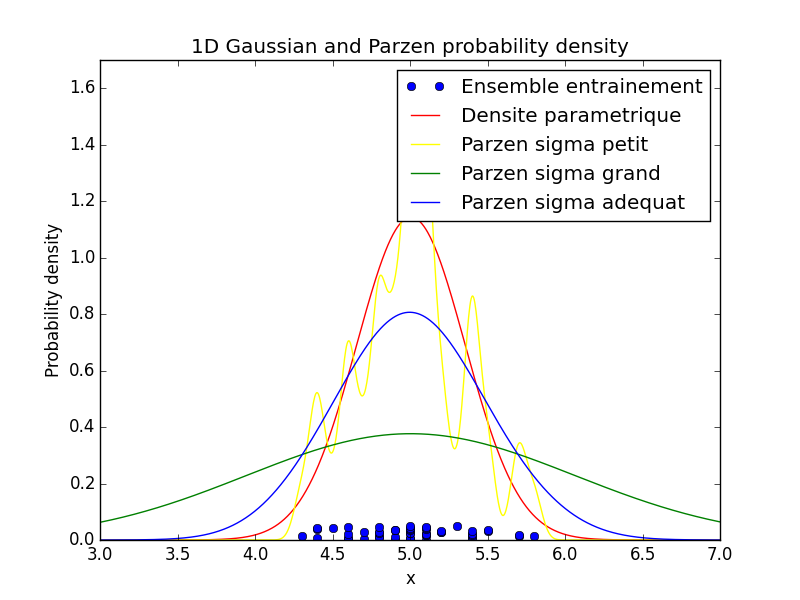
\includegraphics[width=12cm]{images/1D_Gaussian_and_Parzen_probability_density.png} 
	\centering
	\caption{Comparaison de la densité paramétrique et la densité de Parzen avec différents sigma}
	\label{fig:comp}
\end{figure}

\subsection{Densité 2D}

\begin{figure}[H]
	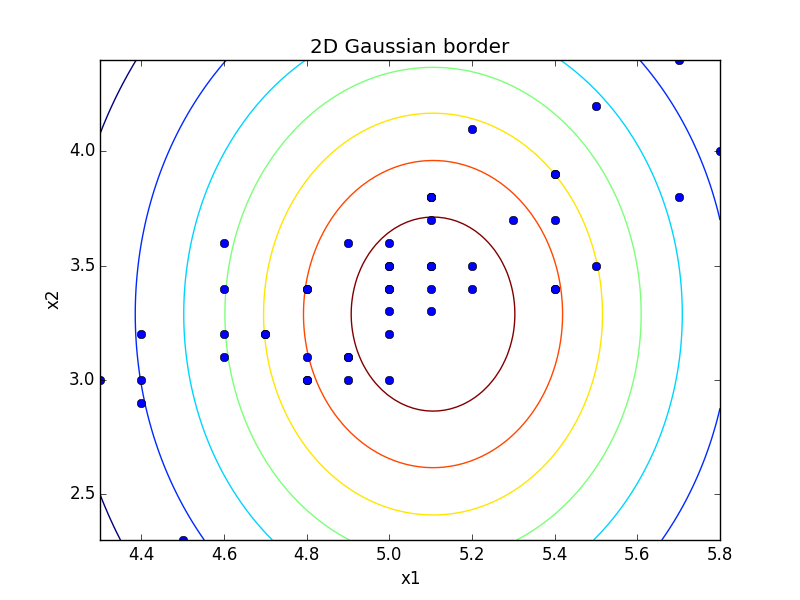
\includegraphics[width=12cm]{images/2D_Gaussian_border.png} 
	\centering
	\caption{Densité paramétrique gaussienne}
	\label{fig:comp}
\end{figure}

\begin{figure}[H]
	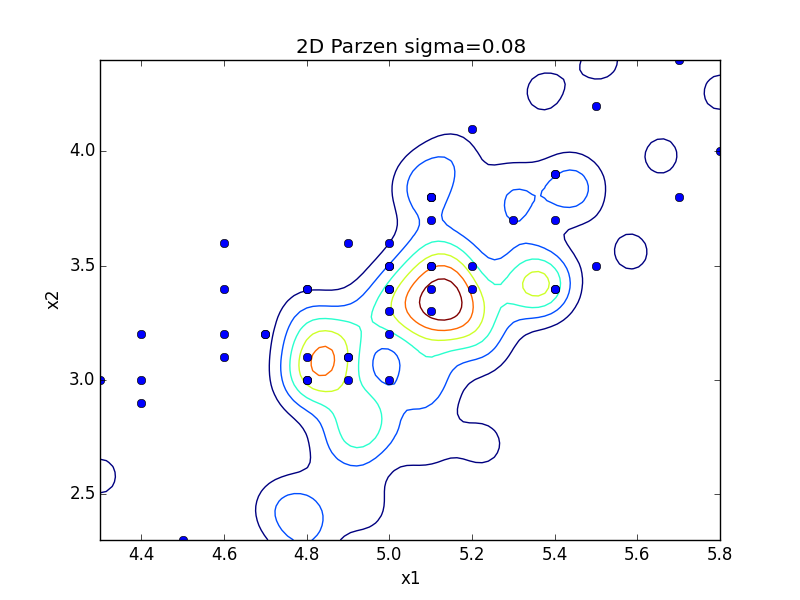
\includegraphics[width=12cm]{images/2D_Parzen_sigma_petit.png} 
	\centering
	\caption{Densité de Parzen : sigma trop petit}
	\label{fig:comp}
\end{figure}

\begin{figure}[H]
	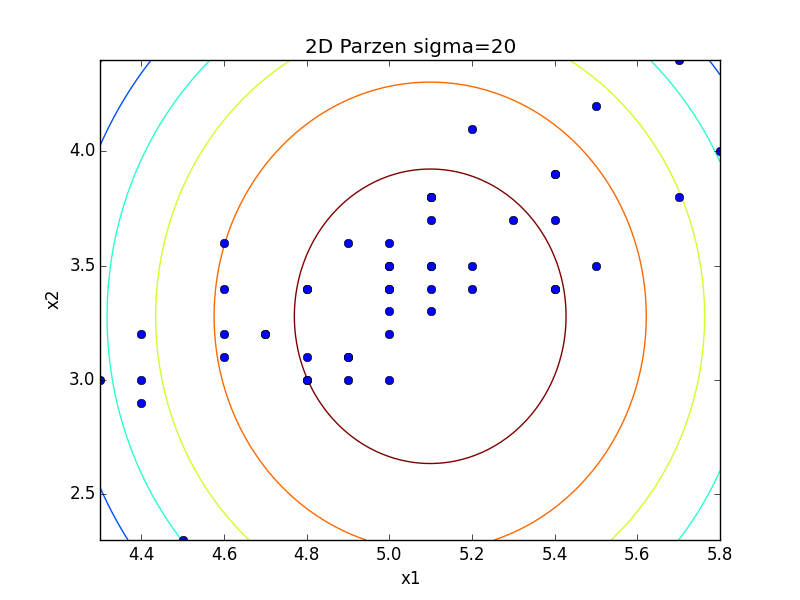
\includegraphics[width=12cm]{images/2D_Parzen_sigma_grand.png} 
	\centering
	\caption{Densité de Parzen : sigma trop grand}
	\label{fig:comp}
\end{figure}

\begin{figure}[H]
	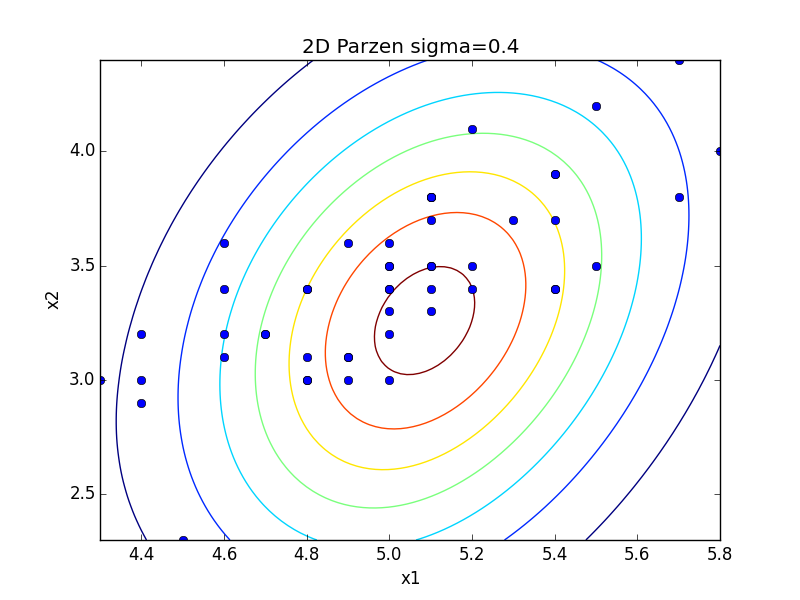
\includegraphics[width=12cm]{images/2D_Parzen_sigma_ad.png} 
	\centering
	\caption{Densité de Parzen : sigma trop adéquat}
	\label{fig:comp}
\end{figure}

\section{Partie Pratique : Estimation de densité}

\end{document}
